% 一维和二维氢原子模型势能
\pentry{定态薛定谔方程\upref{SchEq}}% 氢原子未完成

如果在 1D 或 2D 中直接使用 $V = A/r$ 作为势能, 会发现解不出束缚态.

所以我们一般用 $V_a = A/\sqrt{r^2 + a^2}$ 作为势能, 并且调整 $V_0$ 和 $a$, 使基态等于氢原子的基态. 这个势能相当于把 $1/r$ 势能在原点的奇点变得有限且平滑了, 且 $r\to\infty$ 时有 $V \to A/r$. 当 $a$ 越小, $V_a(r)$ 就越趋近 $V(r)$.

\begin{figure}[ht]
\centering
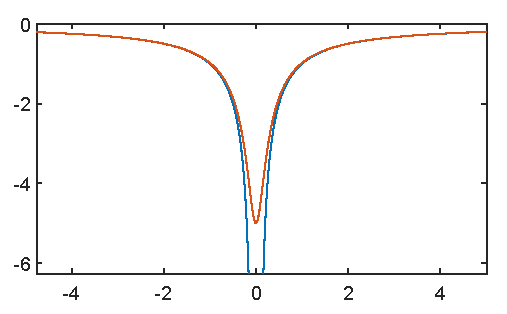
\includegraphics[width=10cm]{./figures/Hy1D2D_1.pdf}
\caption{两种势能的比较, 蓝: $V = 1/r$, 红: $V_a = 1/\sqrt{0.2^2 + r^2}$} \label{Hy1D2D_fig1}
\end{figure}

势能 $V_a$ 没有解析解, 我们只能用数值的方法求解它的束缚态和散射态.
